% !TEX root = ../main.tex
%==========================================%

\section{Introduction}\label{sec:Intro}

Many early cryptocurrency proposals designed secure digital representations of government-issued money (which cryptocurrency enthusiasts typically call `fiat'). While Bitcoin was not the first proposal for a digital currency that is issued and operates independently of existing currencies and financial infrastructure, Bitcoin~\cite{nakamoto2008bitcoin} is the first of this type to establish wide-scale deployment. Without government oversight, the exchange rate of Bitcoin is essentially subject to: (a) an algorithm which releases new BTC (Bitcoin's currency) on a fixed schedule, and (b) the market for exchanging Bitcoin for other things of value, namely fiat currencies such as the USD, and potentially (c) the market for participating in transaction validation which is integral into how new BTC comes into circulation.

%========================%
\begin{figure}[t]
	\centering
	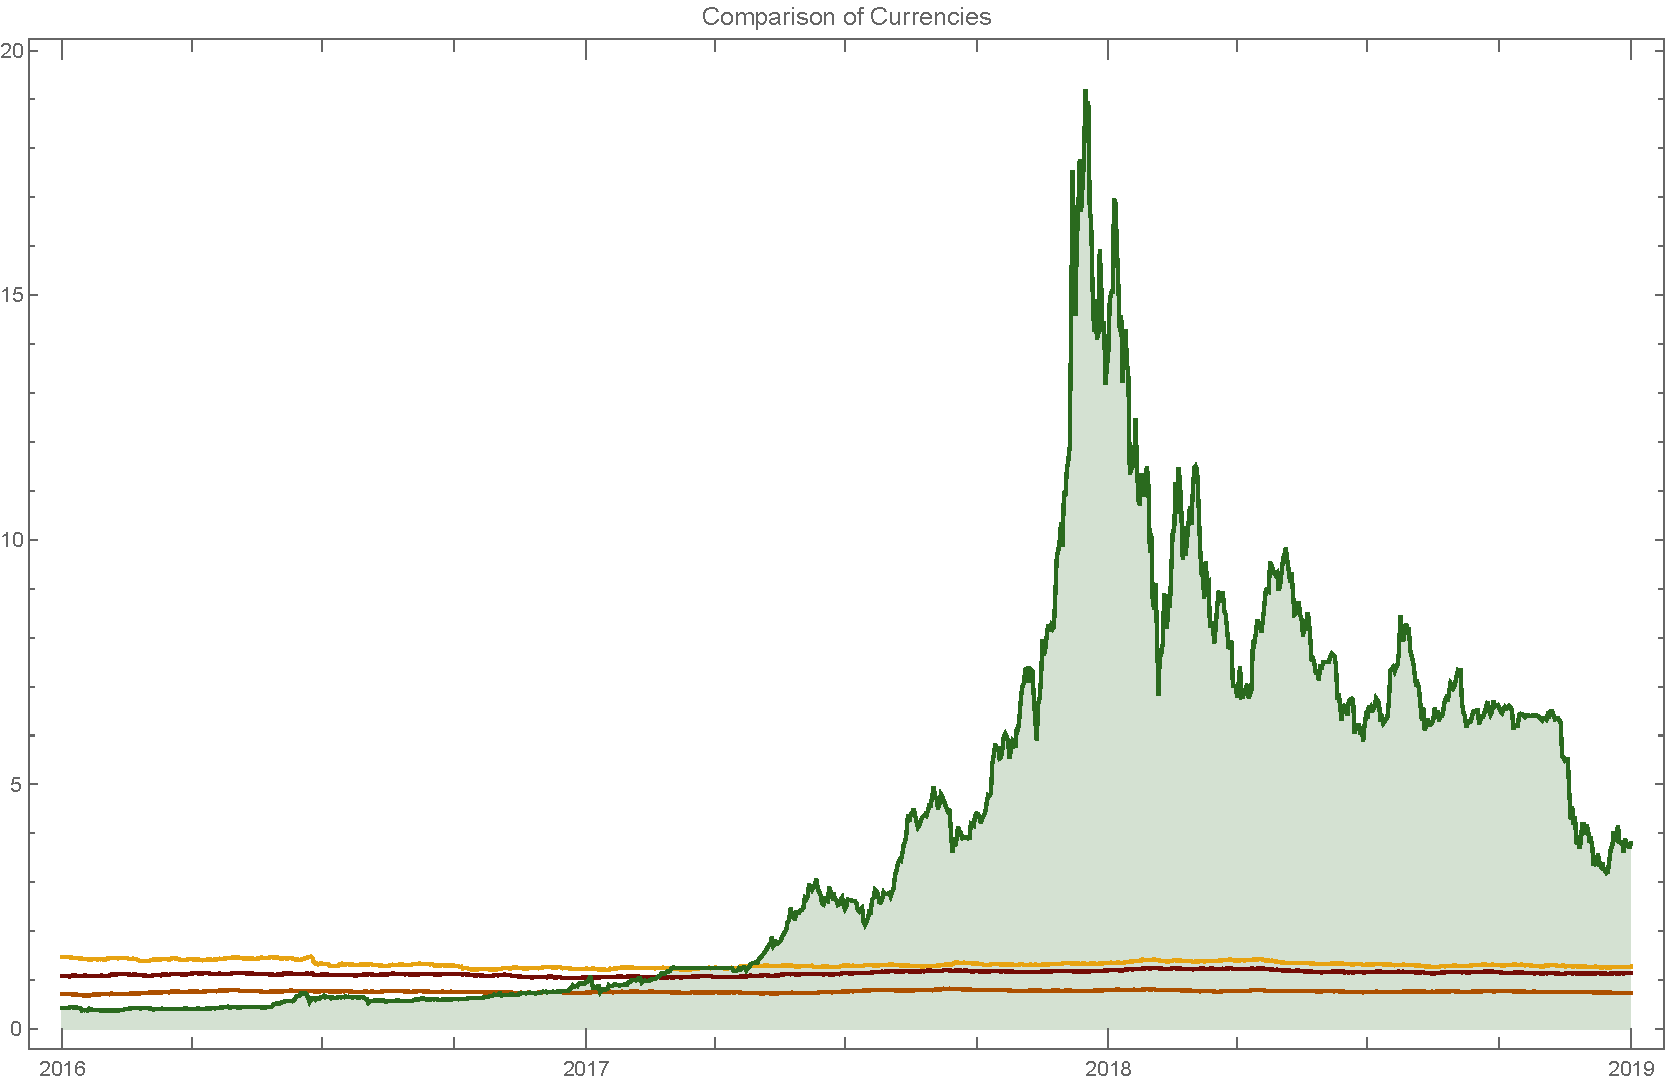
\includegraphics[width=0.8\textwidth]{figures/allCurrencies.pdf}
	\caption{\label{fig:btcandfiat}Comparison among fiat currencies and Bitcoin: The values are retrieved daily between  01 Jan 2016 and 01 Jan 2019. Note that 1000 mBTC = 1 BTC.}
\end{figure}
%========================%

From the inception of exchanges for buying and selling BTC for USD in 2010 to the time of writing, the exchange rate of BTC with the USD has been marked by extremely volatile with large fluctuations in its value that are atypical of a government-managed currency. Figure~\ref{fig:btcandfiat} illustrates this volatility by plotting the exchange rate of BTC (with the USD) alongside the same exchange rate for three economic zones---Europe, UK, and Canada---which all appear relatively stable. Note that Figure~\ref{fig:btcandfiat} deliberately includes the UK's referendum on exiting the EU (`Brexit') in June 2016, which was followed by a `sharp decline' and `volatility' in GBP's exchange rate.\footnote{Descriptions from the following \textit{BBC} articles: ``The markets facing trading turmoil'' (27 Jun 2016) and ``How does Brexit affect the pound?'' (15 Jan 2019).}  Relative to BTC however, this `severe swing' looks like a mild pinch of GBP's exchange rate with EUR in Figure~\ref{fig:btcandfiat}.

In response to Bitcoin's extreme volatility, a flood of proposals have been made for alternative designs that would offer a more stable exchange rate (called `stablecoins') between the newly proposed stablecoin and a government-issued currency like the USD. Broadly, the proposals can be split into two categories: ones that essentially create a digital representation of a currency that can be transacted like a cryptocurrency, and ones that propose separate currencies with some mechanism for stability and/or intervention built into the design.

\paragraph{Contributions.} This paper is essentially a survey of work on stablecoins but we aim at making a number of subtle research contributions to ensure this survey is actually useful to the reader. First and foremost, we are very selective in the concepts from finance we bring into the survey and explain each from first principles, while attempting to minimize or eliminate jargon. Next we distill stablecoin proposals down to a set of fundamental primitives and describe these concepts rather than enumerating the intricate details of how particular `brands' of stablecoins work---details that could change tomorrow. That said, we do provide, as the reader probably expects, a chart mapping existing stablecoin brands into our categorization. Additionally, we also consider the question and potential for the stability of index-cryptocurrencies (namely gas which is used in Ethereum), which are very pertinent to a discussion of stablecoins, yet not typically addressed. Last, we offer a novel visualization style for exchange rates we have not seen before used for exchange rates.

% Most of the coins are mostly focusing on the supporting infrastructure, maybe we also have to talk about the supporting infrastructure of the stablecoin
% Talk about the crypto custodianship somewhere in the paper


\section{Related Work}
\label{sec:lit}

\textblue{there is a lot of different views,  but we should include bank of england(explain that)}
In 2016, Ametrano introduces \textit{Hayek Money}, a new monetary policy of elastic non-discretionary supply that can be used to achieve a price stable cryptocurrency~\cite{ametrano2016hayek}. There are currently many blog posts on the overview of stablecoins and how to design them. According to these resources, the main three approaches to design a stablecoin are (i) fiat-collateralized, (ii) crypto-collateralized and (iii) non-collateralized (also known as algorithmic)(\eg~\cite{hackernoon, comprehensiveOverview, linkedin}) are the examples that give the overview of stablecoins based on these three approaches. \textblue{Note that these resources uses various terms for these three categories interchangeably, \textbf{do we have to mention this? if yes (i) is it the best way of saying it? and (ii) should we mention each and every of these terms? (algorithmic, seignorage shares, elastic money supply)}}
Buterin, in one of the earliest blog posts on stable cryptocurrencies, discussed different techniques to measure cryptocurrencies' price and how to make adjustments in the supply to achieve a fixed price accordingly~\cite{TheSearc7:online}. Bitmex looked at the mechanics of the distributed stablecoins while focusing on two case studies (\ie BitShares (BitUSD) and MakerDAO (Dai))~\cite{bitmex}. Another report from a crypto company called Blockchain \footnote{https://www.blockchain.com} provides an extensive classification of 57 stablecoins together with discussions on issues related to governance (\eg legal structure, investors, partners \etc)~\cite{report}. In one of its blog posts, Consensys \footnote{https://consensys.net} describes stablecoins as "crypto-assets that maintain a stable value against a target price (e.g. USD)" and classify them according to the three main categories~\cite{StateofS96:online}. In~\cite{cryptoinsider}, the authors use a slightly different categorization to group 13 stabelcoin projects into two broad categories: (i) centralized-- which itself contains subcategories based on the type of the asset the coins are backed by (\eg fiat and gold), (ii) decentralized. Unlike other resources that define stablecoins within three categories (fiat-collateralized, crypto-collateralized, and non-collaterlaized), in this paper, we introduce new systemization of stablecoin projects and describe their fundamental primitives.

%=============
% Cite Ross Anderson's paper :"Bitcoin Reducx" :
% Anderson\etal discuss different negative externalities that are introduced by Bitcoin~\cite{anderson2019bitcoin}. They perform and discuss taint tracking using First-In-First-Out (FIFO) algorithm ( inspired by the Clayton’s case) on some well-established Bitcoin theft scenarios. They also point out that crypto space needs effective regulation in order to function properly and securely, at the end they provide regulatory remarks for the future.
%=============
%RSCoin: It is a cryptocurrency framework proposed by Danezis\etal ~\cite{danezis2015centrally}. The supply of money is regulated by a central bank. However, the system depends on a group of distributed authorities to provide transparency and auditability.
%=============

% our chart is basically same as others, but we do different categorization. We all cluster the same way, the main difference is that we strip out the terminalogies, not relying on economic terminologies, we try to represent the difference between these projects. A lot of them leave the readers with the burden of interpretation, things are not clearly defined, except for some technical terms that finance people know. BTW, the table is not our contribution.
% also nobody looked at gas in the context of stablecoin.


%The idea seigniorage shares was first introduced by Robert Sams in 2017, where he proposed a new dual token system that uses two coins to achieve price stability: (i) a stablecoin (\eg fiat currency) and (ii) a volatile coin (\eg equity shares)~\cite{sams2015note}.
%(http://www.andrew.cmu.edu/user/azj/research/rzj_slides201808.pdf): three categories: 100\% USD Reserve backed coins, Protocol coins without redemption, Protocol coins with redemption in floating-rate crypto-currencies
%(https://icosbull.com/whitepapers/2265/USDX_Protocol_whitepaper.pdf) three generations of stablecoins: Collateral-backed IOU, Collateral-backed on blockchain, Elastic monetary supply based. (This is a whitepaper for a protocol but it has a different classification)
%(https://multicoin.capital/2018/01/17/an-overview-of-stablecoins/)  Stablecoins are discussed under three main categories as centralized IOU issuance, collateral backed, and seigniorage shares along with the discussion of different types of oracles and the challenges that stablecoins face.

%=====================Gold vs ETFGold  ===================%
%Gold ETF: Investors want  exposure to the asset that’s electronically traded without taking possession of the commodity.
%advs
% Easy to trade
% No storage and insurance cost
% Hard to steal
% Gold ETF is the most convenient way to store money in gold.
% It is both convenient and low cost. If you’re looking for an inexpensive way to invest in the direction of the gold price, GLD is ideal.
% disadv:
% Ownership of Gold ETFs does not entitle investors to any physical gold.
%  in special occasions when the  market or the bank is not available, the user does not have access to to trade his shares. In this case, ownership of ETF is not any useful for the user.
%  Gold EtTF has counter-party risk and exposed to bad management as the investors have to trust a bank or other trustee to hold and manage their shares
% Physical Gold: Investors want to own the tangible asset
%advs:
% It’s a solid investment and serves as a great hedge against inflation. With strong appreciation through the years, it has proven reliably positive returns even during economic downtimes. Gold prices fluctuate but won’t go away, it won’t be devalued, and it will always be valuable anywhere in the world.
% When you invest in physical gold, you’re entirely in charge of your investment, meaning you’re not trusting it to someone else like an ETF. You decide how to store and secure it.
% When you sell a gold ETF, that data is required by law to be immediately transmitted to the government by the brokerage. Sell gold bullion or bars, and you must report capital gains on your income tax return.
%disadv:
% When you decide to sell your gold, you will have to pay a dealer’s fee as a percentage of your purchase. Hard to buy and sell (trade)
% easy to be stolen
% hard to store


\section{Preliminaries}

\subsection{Prices}

If 1 BTC is worth \$3598.76 USD, as Google says it is at the time of writing, what does that actually mean? There are several subtleties here: (1) what that price actually represents, (2) the relationship between a quoted price and its actual price, (3) the concept that prices are really an exchange of one type of valuable good for another, and (4) the distinction between something's price and its value. The quoted price means that two (hopefully different\footnote{A trade between the same person is called a wash trade and is illegal in most regulated markets.}) people recently exchanged BTC and USD at a valuation of 1 BTC for \$3598.76 USD. First, note that it does not necessarily mean that exactly 1 BTC was exchanged --- it could have been 1 mBTC for \$3.60 or 1000 BTC for \$36M USD. Further, this valuation on the previous trade does not mean you will necessarily be able to exchange 1 BTC for \$3598.76 USD. Last sale price is an indicator of current price that becomes stale as time between subsequent exchanges increase (for example, for a house that last sold 30 years ago, last sale price on a house is not a good indicator of current price).

Instead, we will use the idea of that a cryptocurrency (or any asset) has two prices: (1) the most someone is willing to pay and (2) the least someone is willing to sell for. These are referred to as the best bid price and best ask (or offer) price respectively. Note that the best bid price should logically be less than the best ask price, otherwise an exchange would happen (such prices might occasionally `cross' but this should be temporal and quickly resolved with an exchange). The spread between these prices is called the bid-ask spread.

To understand why this is relevant to stablecoins, consider an example. Say a stablecoin is designed to ensure one unit is always priced at \$1 USD. To argue stability, one must show both that (1) the bid price should never exceed \$1 dollar and (2) the offer price should never dip below \$1 USD. Note, conversely, that bids can dip below \$1 USD (everyone prefers to pay less than something is worth) and asks can exceed \$1 USD (everyone prefers to receive more than something is worth).

\subsection{Exchange Rates}

Consider that several hours after writing the previous section, 1 BTC is now priced at \$3566.56 USD. In one sense, the price of BTC decreased by \$32.20. However it is exactly equivalent to say the price of \$1 USD increased by 0.002 mBTC. This raises a natural question: did BTC decrease in price or did USD increase in price? With an exchange rate, it is impossible to tell. We only know that the price of BTC and USD became closer in price over this short period of time.

To determine which currency is moving, one might consider a third or forth currencies to try and triangulate if BTC is moving in price, or USD is moving in price, or both. For example, in Figure~\ref{fig:btcandfiat} it certainly appears that BTC is the currency that is moving because the rest of the currencies are stable relative to each other. The only alternative is that USD, EUR, GBP, and CAD are volatile currencies that move together as a cluster relative to the stability of BTC. But it is much simpler to conclude that BTC is moving.

%========================%
\begin{figure}[t]
	\centering
	\subfloat[GBP with respect to EUR and USD.]{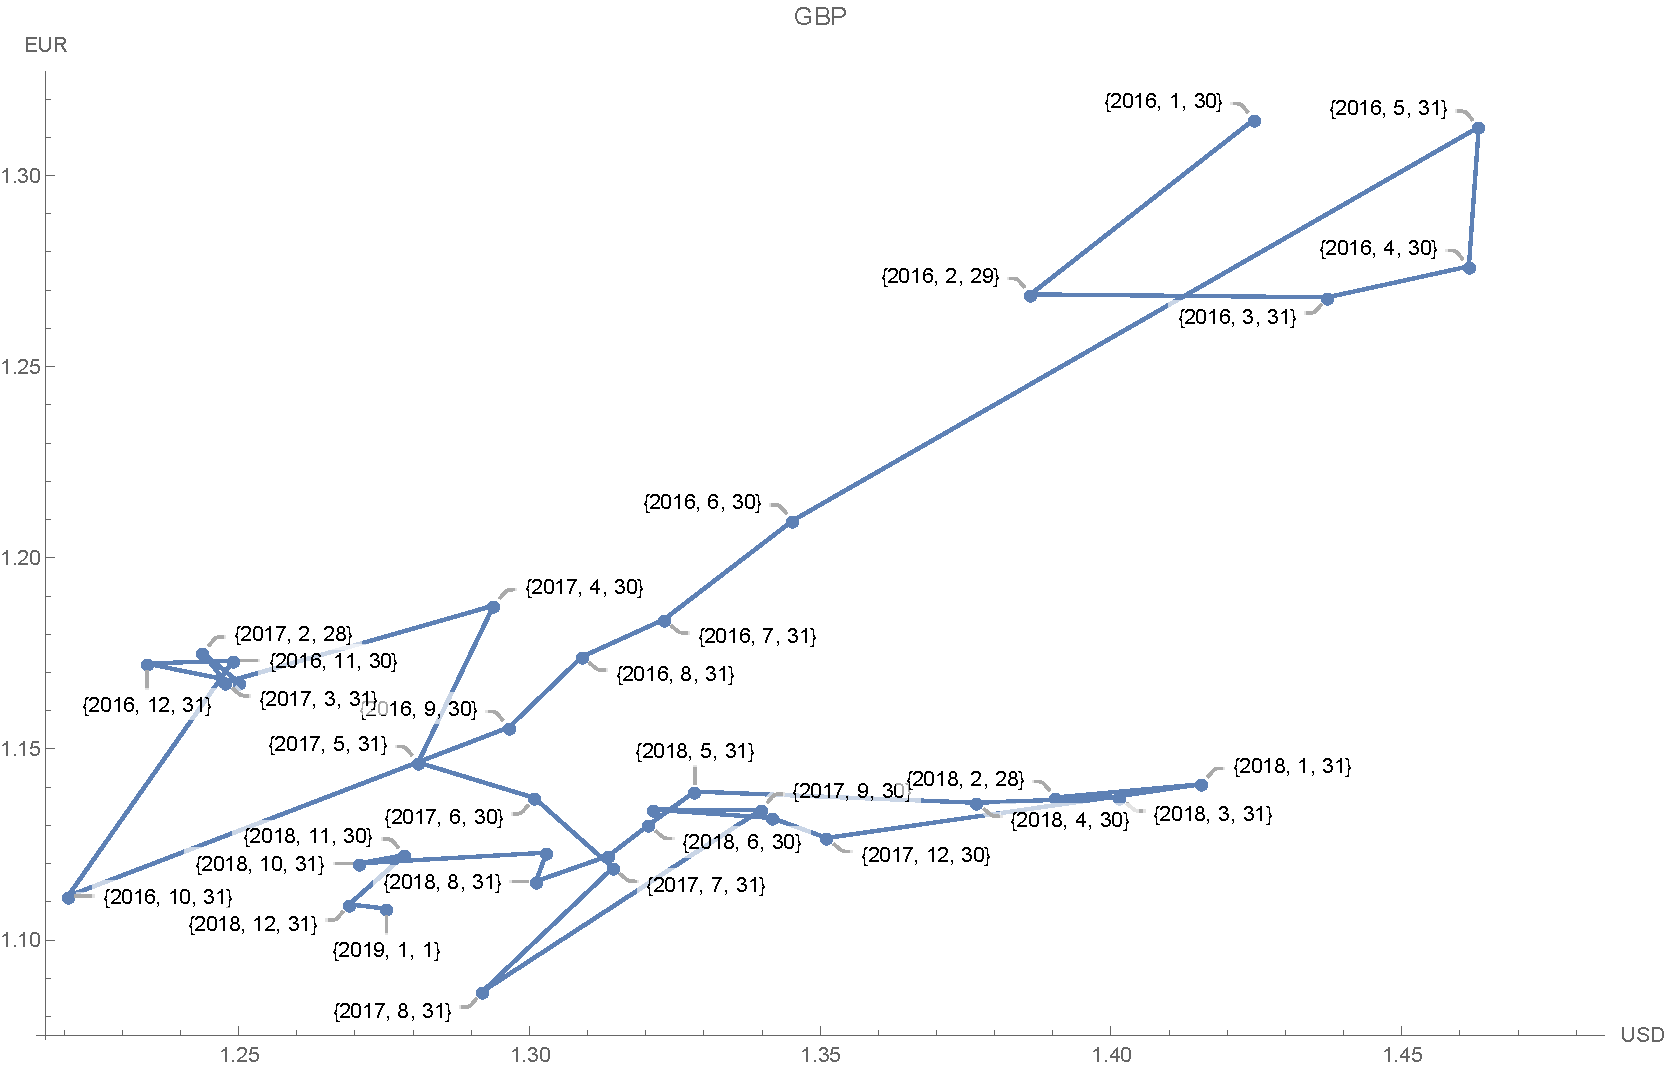
\includegraphics[width=0.75\textwidth]{figures/gbpBrexit.pdf}\label{fig:brexit}}
	\hfill
	\subfloat[Direction labels.]{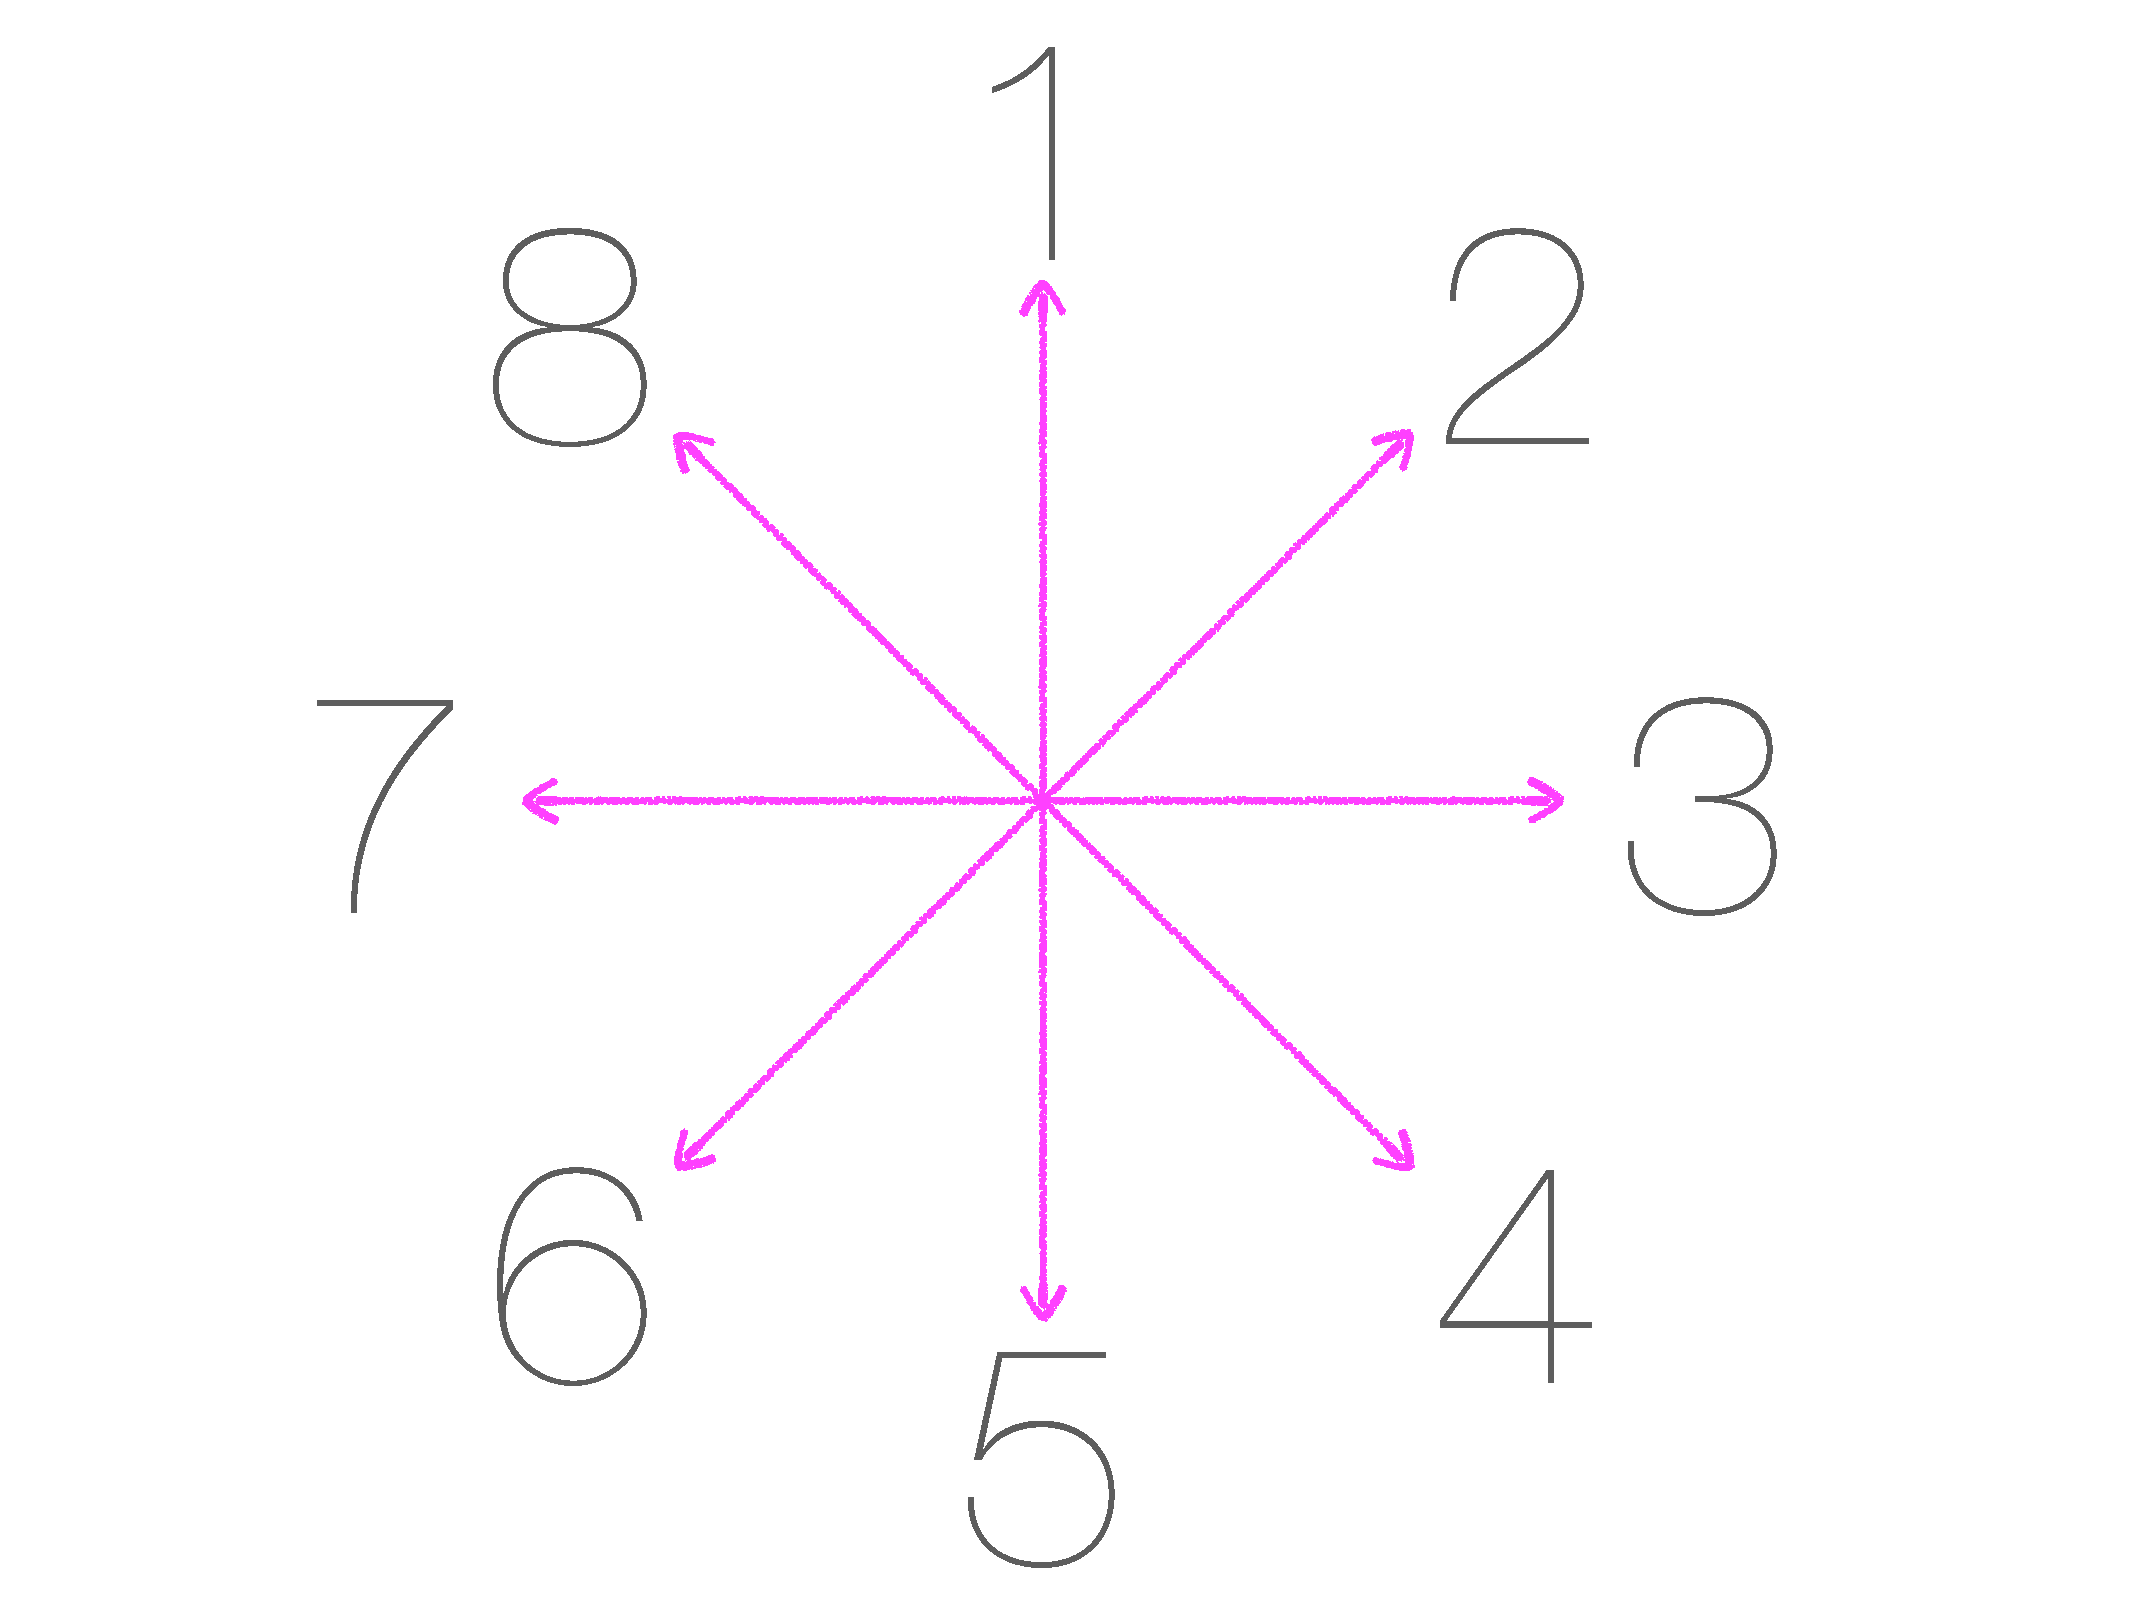
\includegraphics[width=0.25\textwidth]{figures/compass.pdf}\label{fig:legend}}
	\hfill
	\subfloat[The simpliest interpretation of the plots where $X$ refers to the currency on the x-axis (likewise $Y$).]{
	\begin{tabular}{|c|l|}
\hline
\textbf{Direction} & \textbf{Interpretation}   \\ \hline

         1/5                & $Y$ is losing (1) / gaining (5) value \\ \hline
         2/6                & Plotted asset is gaining (2) / losing (6) value \\ \hline
         3/7                & $X$ is losing (3) / gaining (7) value \\ \hline
         4/8                & \multicolumn{1}{p{13cm}|}{Plotted asset is gaining (4) / losing (8) value against $X$, while losing (4) / gaining (8) value against $Y$} \\ \hline

\end{tabular}
	}
	\caption{A connected scatter plot of GBP's exchange rate with EUR and USD demonstrating the effect of Brexit on GBP. Supporting documentation helps interpret the line movements in the plot.\label{fig:Comparison}}
\end{figure}
%========================%

In order to apply this same logic in a visual way, we have created a number of charts like the one provided in Figure~\ref{fig:brexit}. Unlike most exchange rate graphs, these do not use a time axis. Instead each axis is a reference currency. In this case, the price of GBP (plotted value) in USD (x-axis) and EUR (y-axis) forms a coordinate. For the last day of each month, a new coordinate is added and joined with a line from the previous value. This is inspired by similar charts on the website FiveThiryEight for things like kicking distance in football\footnote{``The 52 Best---And Weirdest---Charts We Made In 2016,'' \textit{FiveThirtyEight}, 30 Dec 2016.} and they appear to be called connected scatter plots.

Lines in a connected scatter plot can move in any direction. Figure~\ref{fig:legend} shows how we number the directions from 1 (upward or due north) clockwise to 8 (north-west). For each direction, we describe the simplest interpretation of what that price direction means. By simplest, we mean specifically that we keep an explanation that involves a single currency moving rather than an explanation that involves a pair of currencies moving in tandem. For example, in Figure~\ref{fig:brexit}, GBP shows a drastic movement along direction 6 starting at the time period marked Brexit. This means that GBP is losing value against both EUR and USD. The simplest explanation is that the movements are originating from GBP which is consistent with it losing value after Brexit. Later, GBP shows a lot of horizontal movements along the 7/3 line. The simplest explanation for this segment is volatility in USD rather than GBP.

We will return to these charts later in Section~\ref{sec:stability} where we will use a government currency as one reference (USD on the x-axis) and a cryptocurrency as the other reference (BTC on the y-axis). A stablecoin should exhibit mostly vertical movements along the 1/5 direction.

\subsection{Valuation}

Recall that in the previous section, 1 BTC was priced at \$3566.56 USD. This means that two people recently swapped some amount of BTC and USD for the stated valuation. Does this mean 1 BTC is worth \$3566.56 USD? Value can mean different things in different contexts. The market value of a currency does present one type of value --- its replacement value, or the cost in USD to replace it. Note that more technically, one should  determine replacement value from the set of best offer prices sufficient to cover the volume of BTC being valued.

But does this mean that BTC is fundamentally worth \$3566.56 USD. This is unlikely because by the time you read this paper, the price of BTC in USD is probably quite different from this quoted value (perhaps humorously so). So what constitutes fundamental value? And why do prices change over time?

Stocks, which represent ownership in a firm, and thus a stake in the firm's equity. Therefore shares (called equities) have a fundamental value called its book value: simplified, it is the firm's capital or equity (the value of its assets minus the value of its liabilities, as reported on its annual audited financial statement) divided by the number of outstanding shares. Working in reverse, the price of a single share multiplied by the number of shares represents the market capitalization of the firm. In theory, these numbers should be the same but often are not. When the market capitalization exceeds the reported capital, the market believes the firm's capital will increase over time. If the market capitalization is less than the reported capital, it demonstrates a lack of confidence in the soundness of the firm's financial statements. Floating currencies like the USD, EUR, GBP, and CAD do not have the equivalent of a book value.

To explain Bitcoin's exchange rate with fiat currencies, an oft-repeated theory has emerged that attributes Bitcoin's value to the hydro consumed by blockchain mining. While imprecise, the theory suggests that if a valuable resource $x$ is consumed to produce $y$, the value of $x$ is imparted into $y$. Setting aside the nuance that the hydro contributed to the Bitcoin system only indirectly produces new coins (it produces blocks, and blocks produce coins only for now), there is no economic principle underlying this transfer of value.

%If Alice goes to Peter Luger's in Brooklyn, consumes a \$100 ribeye, and mints a literal shitcoin out of the result --- is that coin worth \$100 because it is ``backed'' by \$100 worth of steak?


\subsection{Stability and Volatility}

When the price of a currency changes over time, it is due to one of two reasons: new information about the currency's fundamental value (even if we cannot concretely say what it is) or transitory volatility due to the trading activites of uninformed traders~\cite{harris2003trading}. For a government issued currencies, information like national inflation rates, macro-economic policies, changes in trade flows, and changes in capital flows seem predictive of changes in the value of the country's currency~\cite{harris2003trading}. Note that a cryptocurrency, like Bitcoin, has none of these indicators. While volatility can be measured mathematically (using variances or deviations), most stablecoins do not offer a concrete, positive definition of what stability means. They tend to be defined by a negative sentiment of what they do not want (the volatility of Bitcoin) rather than a positive sentiment of what they do want.

\subsection{Functions of Money}

There is controversy over whether Bitcoin, and other cryptocurrencies, can even be classified as currencies. The original intent from Bitcoin's creator was for it to be a currency, however it has been assigned many different classifications: from a digitally scarce commodity, to a speculative instrument, to an entirely new asset class.

Most introductory finance textbooks classify currencies according to a set of three core properties it should fulfill for its users. It should operate as a medium of exchange, which roughly means that Alice will accept the currency from Bob because she is confident Carol will later accept it from her. Given the existence of exchange services, Bitcoin is generally considered an acceptable medium of exchange (albeit with some friction). Next, a currency is useful when it serves as the unit of account for pricing other assets. Bitcoin is almost never used as a unit of account and if goods are sold for Bitcoin, it is often priced in, say, USD with a short-lived (\eg 2 minute) spot conversion of the price to BTC for Bitcoin purchases. Finally, currencies should represent a stable store of value. Alice will not accept a currency that depreciates quickly in value from Bob because even though Carol might accept it, what she can obtain from Carol in exchange will be worth less. Less intuitively, currencies that appreciate quickly in value are equally problematic. Alice might gladly accept it from Bob but Bob is unlikely to part with it, and so currencies like this tend to be hoarded. They also hamper lending (see next section).

The goal of a stablecoin is to add the store of value feature to cryptocurrencies, which are already a somewhat adequate medium of exchange. Further, if the currency is stable, it may become a more prominent to use it as a unit of account. Thus stablecoins are intended to make cryptocurrencies more currency-like.

 %Cite Curse of Cash

\subsection{Lending}

Lending a volatile currency poses a risk for both the cash provider and cash taker. Currency depreciation results in the cash provider being repaid less than what they initially provided, and currency appreciation results in the cash taker having to repay a great amount than what was borrowed. Thus a stable currency enables low-risk lending which is beneficial to all participants and is the cornerstone of a modern economy. Okoye \etal put it in a way that is hard to improve on:

\begin{quote}

``It is difficult to overstate the role of lending in a modern economy. Take, as an illustrative example, the role of a central bank; one of the main national institutes (along with the treasury) that cryptocurrencies aim to displace. First and foremost, a central bank is an actual bank, providing accounts for its member banks to deposit money and earn interest. Member banks provide interest-earning accounts to the public. Interest is paid to the public because banks use the deposited money to form loans. Because central bank interest rates are low, banks prefer to lend to other banks any excess cash they hold at day's end instead of depositing them (other banks borrow to meet liquidity requirements). These loans earn interest, and central banks target this specific lending rate when they intervene in the economy. The most common intervention is the buying (circulating new money) or selling (removing circulating money) of government bonds, which are interest-earning loans from investors to the government. Central banks will also provide loans (of `last resort') to banks unable to secure loans from other banks, typically during some sort of liquidity crisis. An economy without loans would have no interest rates, no bonds, and essentially nothing for a modern central bank to do.~\cite{okoyetoward}''

\end{quote}


% = = = = = = = = = = = = = = = = = = = = = = = = = = = = = = = = %

\section{Type 1: Backed Stablecoins}
\label{sec:t1}

In this section, we discuss the first type of stablecoin. These coins try to directly match the stability of a second asset, such as the USD. These coins could not exist without their target asset. In Section~\ref{sec:t2}, we consider the second type of coin which is a standalone currency that use intervention (algorithmic and/or human) to reduce volatility.

% !TEX root = ../main.tex


%-------------------Fancy Table ----------------------%

% = = = Rotated Table Entry \headrow


\newcommand{\headrow}[1]{\multicolumn{1}{c}{\adjustbox{angle=65,lap=\width-0.5em}{#1}}}

% = = = Table bullets: \full and \prt (full and part)

\newcommand{\full}{$\bullet$}
\newcommand{\prt}{$\circ$}
% ------------------------------------------------------------------------------------------------------------------------------------------------%
%Stablecoin projects%

\definecolor{UnitedNationBlue}{rgb}{0.30,0.53,1}
\definecolor{LightSteelBlue}{rgb}{0.69,0.77,0.87}
\definecolor{LightGrey}{rgb}{0.83,0.83,0.83}


\begin{table*}[t]
\centering

\begin{tabular}{|l|l|l|l|l|}

\hline
\rowcolor{lightgray}
\textbf{Class} & \textbf{Mechanism} & \textbf{Resembles} & Rank \\  \hline
% = = = = = = = = = = = = = = = = = = = = = = = = = = = = = = = = = = = = = = = = = = = = = = = = = = = = = = = = = = = = = = = = = = = = = = %
\multirow{17}{*}{Backed}		
						& \multirow{8}{*}{Directly-Backed \& Redeemable$^{\dagger}$}	& USDC 			& 20 \\ \cline{3-4}
						&													& TrueUSD 		& 26 \\ \cline{3-4}	
						&													& Paxos 			& 38 \\ \cline{3-4}		
						&													& Gemini Dollar 	& 52 \\ \cline{3-4}
						&													& StableUSD (USDS) & 685 \\ \cline{3-4}
						&													& Stronghold USD 	& 891 \\ \cline{3-4}
						&													& Petro 			& 1210 \\ \cline{3-4}
						&	& \multicolumn{1}{p{5cm}|}{Ekon, WBTC, emparta} & $\perp$ \\ \cline{2-4}
% = = = = = = = = = = = = = = = = = = = = = = = = = = = = = = = = = = = = = = = = = = = = = = = = = = = = = = = = = = = = = = = = = = = = = = %
						& \multirow{6}{*}{Directly-Backed}  							& Tether 			& 6 \\ \cline{3-4}
						&													& EURSToken 		& 95 \\ \cline{3-4}
						&													& BitCNY 			& 304 \\ \cline{3-4}
						&													& Terracoin 		& 1280 \\ \cline{3-4}
						&													& Saga 			& 1495 \\  \cline{3-4}
						&	& \multicolumn{1}{p{5cm}|}{GJY, Novatti AUD, UPUSD} & $\perp$ \\ \cline{2-4} 						
% = = = = = = = = = = = = = = = = = = = = = = = = = = = = = = = = = = = = = = = = = = = = = = = = = = = = = = = = = = = = = = = = = = = = = = %
						& \multirow{3}{*}{Indirectly-Backed}							& Dai 			& 57 \\ \cline{3-4}
                                                &													& BitUSD 			& 398 \\  \cline{3-4}
                                                & 													& Nomin			& $\perp$ \\ \cline{1-4}
% = = = = = = = = = = = = = = = = = = = = = = = = = = = = = = = = = = = = = = = = = = = = = = = = = = = = = = = = = = = = = = = = = = = = = = %
%						& \multirow{1}{*}{Market Manipulation} 						& NuBits			& 892 \\ \cline{1-4}
\multirow{5}{*}{Intervention}                                                           

% = = = = = = = = = = = = = = = = = = = = = = = = = = = = = = = = = = = = = = = = = = = = = = = = = = = = = = = = = = = = = = = = = = = = = = %
						& \multirow{2}{*}{Money Supply Adjustments}  				& Ampleforth		& $\perp$  \\ \cline{3-4}
						&   													& RSCoin 			& $\perp$  \\ \cline{2-4}
% = = = = = = = = = = = = = = = = = = = = = = = = = = = = = = = = = = = = = = = = = = = = = = = = = = = = = = = = = = = = = = = = = = = = = = %
						& \multirow{2}{*}{Asset Transfer}  							& NuBits			& 892 \\ \cline{3-4}
						&													& CarbonUSD		& 1262 \\ \cline{3-4}
						&													& Basecoin 		& $\perp$ \\ \cline{1-4}
% = = = = = = = = = = = = = = = = = = = = = = = = = = = = = = = = = = = = = = = = = = = = = = = = = = = = = = = = = = = = = = = = = = = = = = %
%						& \multirow{2}{*}{TBD: Internal }  								& Nautiluscoin 		& $\perp$ \\ \cline{3-4}
% = = = = = = = = = = = = = = = = = = = = = = = = = = = = = = = = = = = = = = = = = = = = = = = = = = = = = = = = = = = = = = = = = = = = = = %
\hline
\end{tabular}
\caption{Stablecoin proposals as of January 11, 2019. $\dagger$ \textit{Disclaimer:} Projects are classified according to what they assert; \eg we provide no warranty that projects classified as `redeemable' provide actual redemption of the assets that back their coins. Rank corresponds to \textit{CoinMarketCap}.\label{tab:stablecoins}}
\end{table*}
% ------------------------------------------------------------------------------------------------------------------------------------------------%





In Table~\ref{tab:stablecoins}, we show the taxonomy we use to classify stablecoins. As mentioned earlier in related work (see Section~\ref{sec:lit}), taxonomies for stablecoins have been proposed many times. The focus of our taxonomy is a bit different. We do not care about classification \textit{per se}---we view our work as a tutorial on how to build a stablecoin, and the taxonomy are simply is a set of directions a designer can choose between or combine. They are based on proposals for stablecons, as well as insights from monetary policy for governmental currencies.

To find stablecoin projects, we performed a number of search queries on \textit{CoinDesk}, an online news source for cryptocurrencies and blockchain technology.\footnote{https://www.coindesk.com/} Our search terms included ``stablecoins,'' ``stability,'' and ``price-stable.'' We read 185 articles up to January 11, 2019 and extracted the names of projects. For the 25 projects for which we could find sufficient documentation, we classified them in Table~\ref{tab:stablecoins}. This classification is done according to what the projects assert they do---we provide no warranty of what the projects do in reality. Finally, within each category, we sort projects according to their rank on \textit{CoinMarketCap} which ranks cryptocurrencies that are actively traded on an exchange service.\footnote{https://coinmarketcap.com} Unlisted projects are ranked $\perp$.

% = = = = = = = = = = = = = = = = = = = = = = = = = = = = = = = = %

\subsection{Directly-Backed and Redeemable.}

The first direction one might take in producing a stablecoin is the creation of a digital representation (or tokenization) of a fiat currency, commodity, or portfolio of assets. Tokens are designed to have the same price (and thus volatility) as the underlying portfolio. To further enable an equivalence of value (we will explain how shortly), the digital token can be redeemed on-demand for the underlying asset. For simplicity, we will consider a cryptocurrency designed to digitally represent the USD.

The idea of tokenizing USD (or EUR or gold) for use on the internet is not new. Liberty Reserve and e-gold provided a similar service. Liberty Reserve dollars were redeemable in principle, but only indirectly through an intermediary and redemption could be refused. Meanwhile, e-gold was not redeemable (see next section of a discussion of the consequences of this). What is novel about a stable cryptocurrency is that transactions are not done on a centralized server, but rather finalized and settled on a decentralized blockchain. However since directly-backed stablecoins reintroduce centralization to create the digital tokens, maintain reserves of the underlying asset, and process redemption requests, the benefit of a decentralized transaction platform is marginal.

\paragraph{Process.} Alice is a trusted third party and uses Ethereum to generate a contract to issue 1000 AliceCoins as standard (\eg ERC20) tokens. She lists asks \$1 USD for 1 AliceCoin and promises to redeem the tokens for \$1 USD. If Bob buys 10 AliceCoins for \$10 USD, Alice deposits the \$10 USD in a bank account. Any time Alice receives a request for AliceCoins but does not have any left to sell, she creates new ones and deposits the payment. If Carol wants to redeem 5 AliceCoins, Alice withdraws \$5 USD and exchanges it with Carol and takes the AliceCoins out of circulation. Alice frequently obtains bank statements showing that her account holds USD equivalent to the number of coins in circulation (the number of AliceCoins can be checked anytime on Ethereum).

\paragraph{Price Stability.} For simplicity, assume all transactions are free and frictionless. Consider a bid for 1 AliceCoin that is greater than \$1 USD. Bob will sell an AliceCoin immediately for this price and will ask Alice to generate a new AliceCoin, deposit only \$1 USD for this, and keep the rest of the bid value as profit. Therefore bids in excess of \$1 USD will be temporal assuming Alice is quick to generate new coins on demand. Next, consider an ask for 1 AliceCoin for less than \$1 USD. Bob will immediately purchase this AliceCoin for its asking price, try to redeem it for \$1 USD from Alice, and if successful, keep the difference as profit. Bob's willingness is proportional to the expectation that it can actually be redeemed for \$1 USD. For an example, if he only buys at \$ 0.60 USD, it might reveal that Bob believes there is only a 60\% chance of redeeming the coin or that he can only redeem 60\% of its redemption value (the asker thinks it must be less, otherwise she'd rather redeem it than sell it).

Conclusion: the bid-ask spread will saddle \$1 USD and trades should execute close to \$1 USD assuming the market is close to 100\% confident in a frictionless creation and redemption process for of coins. In reality, fees and time delays for moving stablecoins and fiat payments will cause distortions.

\paragraph{Discussion.} Blockchain-based cryptocurrencies are designed to minimize trust in third parties. The trust assumption on stablecoins in this category are close to pre-bockchain currencies like Liberty Reserve and e-gold, who would maintain transaction details and account balances on a private server. Blockchain enables decentralized trust for the transactions, although it also makes them transparent---at least, as transparent as token movements are for the underlying contract and/or blockchain. This includes transactions with other decentralized applications. However the coin creation and redemption processes rely on trust.

A financial audit is an important step than can establish confidence in the redemption process, which in turns provides stable prices on coins being offered for sale. The auditor becomes a further trusted entity, and ties its reputation to the firm operating the stablecoin. For regulatory reasons, reputable auditing firms will want a clear indication of the coin's legality, as well as confidence in the firm's internal controls over the issuance and redemption of tokens and the custodianship of the backing assets. A sensible template for a stablecoins of this type will consist of three trusted entities: the firm operating the coin, a reputable auditor, and a reputable custodian of the assets.

If the firm operates in a jurisdiction with modern securities laws, the issuance of the stablecoins is likely subject to regulatory approval. Further, the redemption of the coins will serve as a main point of regulation, requiring financial reporting to prevent the kind of crime that was prevalent on pre-blockchain coins like Liberty Reserve and e-gold. A number of existing coins with operations in the United States have been reported as disallowing redemption for some holders.

% According to the recent blogpost in  (https://www.coindesk.com/winklevoss-crypto-gemini-gusd-stablecoin-redemption) Gemini has closed the account of some users and in some cases do not let redemption (some KYC issues) +     Paxos has has the same issue, although they let the user redeem their assets and then closed their account (https://www.ccn.com/paxos-standard-hassling-ethereum-traders-trying-to-redeem-stablecoin-pax-for-dollars)

A variety of firms and projects providing stablecoins in this category exist. Why so many? The differentiation between coins is along a few parameters: (1) the type of asset that can be redeemed for the coin: USD, EUR, gold, \etc; (2) the underlying blockchain (\eg Bitcoin, Ethereum, \etc) and the low-level technical design (updatable contracts, governance, \etc) \textblue{cite that talk on gemini from michael's company's conference}; and (3) the degree of regulatory compliance: paving forward in a highly regulated environment to bootstrap trust, or seeking under-regulated environments to move to market quickly and avoid government surveillance for participants.

% = = = = = = = = = = = = = = = = = = = = = = = = = = = = = = = = %

\subsection{Directly-Backed.}

Next we consider stablecoins that are directly-backed---exactly as in the previous section but they do not offer a redemption process for the coin's underlying assets. Redemption is logistically complicated. Consider a USD-backed dollar---it is usually easier for a firm to receive USD payments from users than it is for it to send payments back, and sending payments opens up new exposure to regulation. Instead, it pledges to keep the backing assets in trust for the duration of the circulating coins. We will shortly explain what impact there is on the coin if it does not provide redemption---obviously, if redemption were inconsequential, than no one would offer it as it increases costs and complexity. For our ranking in Table~\ref{tab:stablecoins}, if we could not find a clear assertion of redemption, we listed the project under this category.

\paragraph{Process.} As previously, Alice is a trusted third party and uses Ethereum to generate a contract to issue 1000 AliceCoins as ERC20 tokens. She asks \$1 USD for 1 AliceCoin and promises to deposit the payment. If Bob buys 10 AliceCoins for \$10 USD, Alice deposits the \$10 USD in a bank account. Any time Alice receives a request for AliceCoins but does not have any left to sell, she creates new ones and deposits the payment. Alice frequently obtains bank statements showing that her account holds USD equivalent to the number of coins in circulation (the number of AliceCoins can be checked anytime on Ethereum).

\paragraph{Price Stability.}

\paragraph{Discussion.} The idea of tokenizing assets and re-selling them in a useful format (\eg as a portofolio or in a way that is digitally compliant with standard trading software and automated accounting systems) is commonplace for standard financial assets, however most tokenizations of this type have some direct or indirect redeemable value. An electronically traded fund (ETF) will typically sell shares of a portfolio of assets, be redeemable for the assets, and will be priced closely ($\pm 1\%$) to the value of its underlying assets---it is most like the stablecoins in the previous section. A simplification of a trust fund, such as a closed end fund, is as follows: a firm will set up a special corporation to hold the assets, the tokens are not directly redeemable, however the tokens are ownership shares in the special corporation---by owning the corporation, you effectively own its assets. Such a fund will be more moderately priced ($\pm 5\%$) to the value of its assets. \textblue{Need to distinguish out three cases: directly redeemable, redeemable for ownership, not redeemable at all}.

% Description of how it works. Deposit in bank, etc.
% Regular audits are needed to ensure that the stablecoin is indeed fully collateralized
% Justification that bids will never exceed $1:
% Justification that offers will be less than $1
% Examples: Tether
% Remarks:

% Discussion: ETF are 1\%, CEF are 5\% but CEF still gives you equity in the SPV holding the funds, redemption is point of regulation
% Tether attacks
% imparted attacks

% = = = = = = = = = = = = = = = = = = = = = = = = = = = = = = = = %

\subsection{Indirectly-Backed.}
% Description of how it works.
% Justification that bids will never exceed $1
% Justification that offers will be less than $1
% Examples:
% Remarks: Oracles

% = = = = = = = = = = = = = = = = = = = = = = = = = = = = = = = = %

%There is middle category of redeemability.
%similar to indirect owership of gold. It is redeemable for a share of the company that holds the gold.
%check the backed ones for having shares or not

\section{Type 2: Intervention-based Stablecoins}
\label{sec:t2}


% Control system: input (metrics), make a decision, implement the intervention
% We cannot prove that something here works or not. It is all heuristics. We know this because central banks themselves operate on heuristics that change every couple of decades. Even if we cannot say something does work, we can point out a few suggestions that it will not work. Game-able inputs, inputs/interventions that have not worked for currency.

% = = = = = = = = = = = = = = = = = = = = = = = = = = = = = = = = %

\subsection{Market manipulation}

% Description of how it works.
% Justification that bids will never exceed $1
% Justification that offers will be less than $1
% Examples:

%=================%
%IMF's papers on currency boards(https://www.imf.org/external/pubs/ft/pdp/2000/pdp01.pdf):one of the elements in a currency board: fixed exchange rate pegged to a foreign anchor
%aim: monetary stability and low inflation
%currency board needs sufficient backing of base money (=central bank holds sufficient foreign exchange reserve)
%CBA has adjustment mechanism. It reacts automatically to the changes in the foreign exchange outflows and inflows.Interest rates adjust automatically in currency board based systems
%problem when the domestic inflation rate is higher than the inflation rate of the underlying foreign currency: results in overvaluation of the domestic currency

%(https://www.imf.org/external/pubs/ft/wp/wp9808.pdf): Difference between currency board and pegged exchange rate
%=================%

%Interest rates: borrower pays her loan + interest
%Negative interest rate: borrower is paid the interest + she uses the loan
%Sweden and Japan are examples of countries that use NIR

% = = = = = = = = = = = = = = = = = = = = = = = = = = = = = = = = %

\subsection{Discretionary input; money expansion/contraction output}

% Description of how it works.
% Justification that bids will never exceed $1
% Justification that offers will be less than $1
% Examples: RSCoin

% = = = = = = = = = = = = = = = = = = = = = = = = = = = = = = = = %

\subsection{Money expansion/contraction}

%Intro

\paragraph{Process.} Alice forks Bitcoin to create a new altcoin called AliceCoin. She sets Bitcoin's fixed schedule for releasing new Bitcoin as the default behaviour but allows this value (called the coinbase amount) to be tweaked according to the rules outlined below. She setups up a trusted oracle for the latest exchange rate of AliceCoins to USD. AliceCoin is programmed to apply an intervention when the price of an AliceCoin exceeds \$1.02 USD or dips below \$0.98 USD. If the price exceeds \$1.02 USD, the miner is allowed to increase the coinbase amount (the amount is determined by some mathematical relationship with how much the price exceeds \$1.02 USD). If the price dips under \$0.98 USD, the miner must decrease the coinbase amount (again, based on some mathematical relationship). The correctness of the claimed coinbase is verified by other miners in deciding to accept or reject a mined block, as per all other checked conditions in Bitcoin.

\paragraph{Variant.} Similar to above, Alice forks Bitcoin, preserves its coinbase schedule, and adds a trusted exchange rate oracle. When the price exceeds \$1.02 USD, the coin increases the balance of every AliceCoin holder; when it dips below \$0.98 USD, the coin decreases the balance of every AliceCoin holder.

% Zero bound -> actually maybe not: Miner gets Reward + Fees, reward can be negative if fees are larger and difference is removed from circulation. -> pushing volatility into fees
% Ambleforth -> just take currency from holders.

% Description of how it works.
% Justification that bids will never exceed $1
% Justification that offers will be less than $1
% Examples: RSCoin

\subsection{Indirect money expansion/contraction}

\paragraph{Process.} Alice creates an ERC20 token called AliceCoin and setups up a trusted oracle for the latest exchange rate of AliceCoins to USD. A smart contract is programmed to apply an intervention when the price of an AliceCoin exceeds \$1.02 USD or dips below \$0.98 USD.  If the price exceeds \$1.02 USD, the contract creates new a set of AliceCoins (the size is determined by some mathematical relationship with how much the price exceeds \$1.02 USD) and transfers them to users waiting in line for them. How do users wait in line? When the price dips under \$0.98 USD, the contract creates new positions at the end of the line and auctions them off to the highest bidder. The payment for a place in line is made in AliceCoins from the bidder to the contract and the contract destroys the payment. The place in line is a transferrable token. An additional transferrable token can be auctioned off which receives AliceCoins when the line is empty.

% Description of how it works.
% Push volatility around -> into bonds which flucuate from deep haircut to \$1 USD

\paragraph{Price Stability.}
% Justification that bids will never exceed $1
% Justification that offers will be less than $1
% Examples:

\paragraph{Discussion.}
% Push volatility around
% \textblue{Ethereum Alarm Clock problem.}

% = = = = = = = = = = = = = = = = = = = = = = = = = = = = = = = = %

\subsection{Blockchian metrics input; with only internal information}
% Description of how it works.
% Justification that bids will never exceed $1
% Justification that offers will be less than $1
% Examples:


%================Notes on unranked projects:==========================%

%CarbonUSD:
%t hybridizing both fiat backed and algorithmic stablecoins, (hybrid fiat-algorithmic approach)
% 1-1 backed with USD
% unlike purely fiat-backed stablecoin, CarbonUSD's novel meta-token structure enables a seamless future transition to an algorithmic stablecoin model once it reaches sufficient scale as a fully fiat-backed token.
% meta-token smart contract is a key innovation that enables carbonusd to eventually transition from full fiat-collateralization without distrupting its liquidity network effects on exchanges and while maintaining the highest standards for regulatory compliance.
% HOW? CarbonUSD is a basket of whitelisted tokens. A token that is whitelisted may be used to create new CarbonUSD, serving as its collateral. Initially, only one token will be whitelisted, a stablecoin that is 1-1 backed with USdollars in a trust account.
% The first whitelisted token, WT0, is a compliant fiat-backed stablecoin where users can deposit and withdrawal real USD. Governing members of the whitelist can decide when CarbonUSD has enough liquidity to safely switch off from full fiat- collateralization.
% they also have regular audits (unlike Tether)
% Redeemable
% Offchain (fiat-backed, crypto-backed) stablecoins are effective as bootstrapping trust and NOT maintaining it scale. HOWEVERM, Onchain (algorithmic) stablecoins are effective at maintaining trust at scale BUT not at bootstrapping it.
%=================%
%NuBits:  https://nubits.com/NuWhitepaper.pdf
% Like Tether, NuBits are pegged to US dollar, with one dollar equivalent to one NuBit.
% NuBits controls its coin's value by getting shareholders to place buy and sell orders at 1$ for NuBits, rewarding them with revenue from sales of NuBits external cryptocurrency, NuShares.
%==========
% NuBits has suffered two big crashes, with extended peg breaking.
% First :
% In 2016, NuBits’ peg infamously broke, and it remained broken for 3 months. The initial price drop happened between May 26th and June 20th, 2016. This was about the same time that Bitcoin’s price suddenly spiked, after 6 months of relative stability. It’s plausible that the drop happened because of the following: People who had capital in NuBits saw how Bitcoin was spiking. They wanted to get in on the spike, so they sold their NuBits in large quantities to buy Bitcoin. The NuBits peg was unable to handle the large sell-offs and broke. The price tanked and the peg stayed broken for an extended period. It seems that when the Bitcoin and volatile cryptoassets’ prices spike, investors with capital in stablecoins will want to sell them off to get in on the spike. That causes strong downward pressure on the stablecoin price.
%==========
% Second:
% After NuBits crashed in 2016, its market cap grew 1,500% on Coinmarketcap between the end of 2017 and the beginning of 2018, going from $950k to $14 million. This is strange, considering the NuBits peg had been broken for such a long period in 2016. Their market cap had been stagnant for years, and suddenly it takes off. Was this spike just an accounting error, or had people suddenly decided NuBits was actually amazing?
% Turns out the increase was real. However, it did not happen in one day. People were buying millions of NuBits in late December. The price of the NuBits stablecoin was notably above its $1 peg between December 20 and December 28, when it peaked close to $1.50(!).
% What caused the increase? It’s clear when one looks at the Bitcoin price history. The NuBits high price period starts when Bitcoin had its “Christmas crash.” By December 22 there was a strong news narrative about Bitcoin crashing.
% As long as there was a lot of uncertainty about Bitcoin’s stability, people kept buying large numbers of NuBits. Then, by the New Year, when Bitcoin temporarily normalized again, the large NuBits buy-ins stopped.
% What happened, then? Well, Bitcoin holders noted the dropping Bitcoin prices and got worried about an imminent crash. Converting BTC to USD is slow and can lead to taxation. So the worried Bitcoin holders converted their crypto assets to stablecoins rather than cash. Some choose NuBits. The very large influx of Bitcoin money doubled the NuBits market cap several times over. The NuBits folks were frantically printing new money and selling it off to the Bitcoin holders. But demand was so great among panicked Bitcoin holders that the new NuBits couldn’t be printed fast enough and their price was driven up high.
% This shows how when Bitcoin and cryptomarkets crash, capital rapidly flows into stablecoins.
%==========
% NuBits sounds very much like Basis: When the price of the Basis token below 1 dollar, they start selling sth called a bond token, and they actually sell this at a price below 1$ with a promise that it can be redeemed for a Basis coin in the future. when the price of Basis token goes above 1$, the Basis algorithm has to increase the money supply, so tehy issue you a 1 to 1 Basis coin for each Basis bond token that you held.
%=================%
%Ampleforth:
% It uses a different method of preserving its dollar-to-unit ration, by transferring volatility from unity price to unit count.
%According to Trail of Bits, a malicious market maker could play with the stability of Ampleforth. the issue is their oracle services use whitelisted sources (just like Dai)
%=================%
%Havven
% is mostly like Dai, they also use over collateralization with 1:5 ratio.
% They use a similar arbitrage as Dai but with different functionalities by locking up Havven tokens or by reverse burning Nomins by reclaiming Havven tokens  to keep the price stable.
% One key difference between Nomin and Dai is the collateral for Dai is Eth but for Nomin is the actual Havven token itself.
%=================%
%Basecoin (Basis Algorithm)
% Non-collateralized
% Controlled by algorithmic supply
% The price  stability of this coin is managed by Basis protocol which is a central bank algorithm that increases or decreases the supply of teh coin based on supply and demand
% Still experimental and not yet operational
 % The coin supple is entirely done based on the information given by differnt oracles that make the protocol aware of condition of supply and demand
 % The peg could be anything: fiat, assets, or a basket of assets

%==========================================%
\section{Evaluation Framework}

In this Section, we review various issues with different mechanisms of designing a stablecoin (discussed in Sections~\ref{sec:t1} and~\ref{sec:t2}) . We provide an evaluation framework based on x (\textblue{to be filled}) criteria (see Table~\ref{tab:evframework}) that evaluates each mechanism's core ideas and trust model. The columns and rows of the table are the evaluation criteria and mechanisms respectively. This framework provides a summary of advantages and disadvantages of different mechanisms for creating stablecoins.


%===========Version1============%

%\begin{table}[t]
%\centering
%\begin{tabular*}{0.9\textwidth}{@{\extracolsep{\fill}} lccccccccc}
%
%&
%&
%&
%\headrow{Stable to undervaluation} &
%\headrow{Stable to overvaluation} &
%\headrow{Issuance is decentralized} &
%\headrow{Redemption} &
%\headrow{Transfer} &
%\headrow{Oracle} &
%\headrow{Risks} \\
%
%\hline
%
%\textit{Class} &\textit{Mechanism}&\textit{Resembles}&  \multicolumn{2}{|c|}{Stability} &  \multicolumn{4}{c|}{Trust} &  \multicolumn{1}{c}{Risks} \\
%c
%\hline
%
%\multirow{3}{*}{Backed}                                                         \\
%& \multicolumn{1}{c}{Directly Backed and Redeemable}	       \\
%&\multicolumn{1}{c}{Directly Backed}                                     \\
%&\multicolumn{1}{c}{Indirectly Backed}                                     \\
%\hline
%\multirow{5}{*}{Intervention}                                                        \\
%&\multicolumn{1}{c}{Currency Board}                                         \\
%&\multicolumn{1}{c}{Contract Expand }                                       \\
%&\multicolumn{1}{c}{Managed}                                                    \\
%&\multicolumn{1}{c}{seignorage Shares}	                                     \\
%&\multicolumn{1}{c}{Internal}                                                        \\
%\hline
%
%\end{tabular*}
%\caption{Evaluation Framework Version 1.\label{tab:evframework}}
%
%\end{table}
%===============Version2===================%
\newcolumntype{N}{>{\centering\arraybackslash}m{.45in}}

\begin{table}[htb!]
	
	\begin{tabular*}{0.9\textwidth}{@{\extracolsep{\fill}} lllllllll}
		
		&
		&
		\headrow{Stable to undervaluation} &
		\headrow{Stable to overvaluation} &
		\headrow{No issuance violation} &
		\headrow{Redemption guaranteed} &
		\headrow{No intermediaries for transfer} &
		\headrow{No trusted oracle} &
		\headrow{No collateral termination} \\
		
		\hline
		
		\textit{Mechanism}  &   \textit{Resembles}  &  \multicolumn{2}{|c|}{Price Stability} &  \multicolumn{4}{c|}{Trust} &  \multicolumn{1}{c}{Risks} \\
		
		\hline
		
		Directly Backed and Redeemable	 &  & \multicolumn{1}{|c|}{\full } & \multicolumn{1}{c|}{\full }   & \multicolumn{1}{c|}{ } & \multicolumn{1}{c|}{} & \multicolumn{1}{c|}{} & \multicolumn{1}{c|}{} &   \\
		Directly Backed                                 &  & \multicolumn{1}{|c|}{\full } & \multicolumn{1}{c|}{}   & \multicolumn{1}{c|}{ } & \multicolumn{1}{c|}{} & \multicolumn{1}{c|}{} & \multicolumn{1}{c|}{} &   \\
		Indirectly Backed                                &  & \multicolumn{1}{|c|}{\full } & \multicolumn{1}{c|}{}   & \multicolumn{1}{c|}{ } & \multicolumn{1}{c|}{} & \multicolumn{1}{c|}{} & \multicolumn{1}{c|}{} &   \\
		Currency Board                                  &  & \multicolumn{1}{|c|}{\full } & \multicolumn{1}{c|}{}   & \multicolumn{1}{c|}{ } & \multicolumn{1}{c|}{} & \multicolumn{1}{c|}{} & \multicolumn{1}{c|}{} &   \\     \hline
		Contract Expand                                  &  & \multicolumn{1}{|c|}{\full } & \multicolumn{1}{c|}{}   & \multicolumn{1}{c|}{ } & \multicolumn{1}{c|}{} & \multicolumn{1}{c|}{} & \multicolumn{1}{c|}{} &   \\
		Managed                                             &  & \multicolumn{1}{|c|}{\full } & \multicolumn{1}{c|}{}   & \multicolumn{1}{c|}{ } & \multicolumn{1}{c|}{} & \multicolumn{1}{c|}{} & \multicolumn{1}{c|}{} &   \\
		Seignorage Shares	                               &  & \multicolumn{1}{|c|}{\full } & \multicolumn{1}{c|}{}   & \multicolumn{1}{c|}{ } & \multicolumn{1}{c|}{} & \multicolumn{1}{c|}{} & \multicolumn{1}{c|}{} &   \\
		Internal                                                    &  & \multicolumn{1}{|N|}{\full} & \multicolumn{1}{c|}{}   & \multicolumn{1}{c|}{ } & \multicolumn{1}{c|}{} & \multicolumn{1}{c|}{} & \multicolumn{1}{c|}{} &   \\
		\hline
		
	\end{tabular*}
	\caption{Evaluation Framework Version 2.\label{tab:evframework}}
	
\end{table}
%=============%
%About the evaluation Framework:
%Stability
%-----------
%Is the currency stable to undervaluation?
%Let's say, I buy a token for 80 cents and sell it for 1 dollar (which means the token is redeemable), then  I profit; but if it is not redeemable than I can't do this.
%The problem with undervaluation is that I may end up not being able to redeem my token for the underlying currency.
%
%Is the currency stable to overvaluation?
%I buy a token for 1 dollar and if someone wants to buy it for 1.30, I profit.
%
%Trust
%------
%Does the token requires trust in a central party (for example to keep the required amount in reserves to back the coin)?
%I need to be able to trust the system that it won't issue many tokens, so that the token deflates eventually.
% Do I trust you'll issue right number of tokens?
%About transfer: liberty reserve, egold similar to tether only difference is that Tether is decentralized
%in order to redeem whom should I trust?
%Is there an oracle feed for determining the exchange rate?
%
%Risk
%-----
%For Dai: the underlying cdp can lose its value and the coin cannot be redeemed. About time sensitivity, semi-redeemable (there is a risk of not being able to redeem)
%========
%Directly-backed and redeemable:
%Stability:
%It is stable to undervaluation, as it is redeemable
%overvaluation??
%Trust:
%Needs to trust a central party for issuance and redemption
%Directly backed:
%not stable to undervaluation because it is not redeemable. So, if I buy a token for 80 cents and can't redeem it back for 1 dollar (which is the promised price for the token by the system), then I cannot profit.
%
%
%full circle: the property is achieved
%empty cell: the property is not achieved
%empty circle: the property is partially achieved
%-: not applicable

\section{Discussion}

\subsection{Why so many?}

%Emphasis on other things, like setting up contracts, governmence, audits, etc.
% Which blockchain

\subsection{What Stability looks like}\label{sec:stability}
\subsection{Ethereum's Gas}\label{sec:GasInvs}
% Gas: non-redeemable backed by Ether. like putting Ether in the contract and get USD digital token. why non-redeemable? because you burn Gas to get your digital tokens.
% Depending on how much the user wants to pay for ecah unit of Gas, this will determine how expensive the tx is in Ether.
% Gas is internal to the Ethereum blockchain and users cannot hold it, instead they can have Ethere, BUT the conversion rate between Gas and Ether changes over time and that's why there are huge spikes in the average Gas price plots.
% But we can make Gas redeemable, there is a way in Ethereum to do that, the GasToken that uses this strategy. It allows you to stockpile and trade Ethereum Gas.
% Gas is not a currency so you cannot buy things with it BUT you can turn it into a currency : having a smart contract and swaps it with other tokens
% Gas is actually stable with respect to others, the reason it's not obvious is human error and their wrong mental model
% Gas is not pegged to anything
% Gas is free floating but it’s driven (governed) by market forces (auctioning off)
% there is an upper band and lower band for Gas
% So in this section we look into how to trade Gas and its derivatives?

%=======GasToken details=======%
% Operations that modify the global state of the Ethereum blockchain are very expensive \ie writing into a contract storage.
% Ethereum motivates the user to free up space on the blockchain by refunding the Gas if they delete their contracts. This is what GasToken does.
% GasToken is a smart contract that for the first time allows Ethereum users to buy and sell gas by tokenizing gas on the network. \footnote{https://github.com/projectchicago/gastoken}
% They allow users to store Gas when it is cheap and use it once its price goes up.
% Gas price refers to the amount of Ether you’re willing to pay for every unit of gas.
% When a user stores cheap Gas, he can later spend that Gas to send a tx, that means now he pays for less gas for that tx to go through.
% GasToken allows a transaction to do the same amount of work and pay for less gas, saving on miner fees and costs and allowing users to bid higher gas prices without paying correspondingly higher fees.
%The gas tokens works on taking advantage of storage refund concept in ethereum, to inspire smart contracts to delete storage variable, ethereum network provides refund when storage variable is deleted up to half of the contract transaction.
	% If a variable is changed from zero to a non-zero value, there is a gas fee  (writing into the storage is a very very expensive operation because it's altering the global state)
	% If a variable is changed from a non-zero value to zero, there is a gas refund
% A user can:
	% Mint tokens when GasPrice is low: change a variable from a zero value to non-zero.
	% Burn tokens when GasPrice is high: change a variable from non-zero to zero.

% As mentioned, the gas refunded from freeing some storage space is less than the initial gas cost of storing the data on-chain in the first place, so why would someone want to do this? Well, you can create these GasTokens (filling an array with ones or creating a bunch of contracts) at a time t with a low gas price (e.g. 2 Gwei) and later consume these GasTokens in a transaction that has a higher gas price. Hence, half of your gas used for the expensive transaction effectively costs you 2 Gwei, while the other half costs 50 Gwei. Even if you don’t get back as much gas as you spent creating these GasTokens, the difference in gas price can make it worth it.

% IMPORTANT: How is the mechanic? 1) when the Gas price is low, user calls the gastoken contract and asks it to store a bunch of words, this costs a lot of gas but because gas is cheap it will only cost a few cents for the user. 2) later in the future, where the user wants to register a domain and the gas price is so expensive, user will create a tx and within that he does 2 things: (i) register the domain she wants and (ii) ask gastoken contract to remove those words she's stored before.

%=================%
% Freeing up many storage slots in one transaction can quickly result in the refund counter surpassing half of the full transaction cost. In such a case or in case of self-destructs which can lead to a high refund counter as well we should evaluate how much of the refund can actually be used, as the refund can be at most half of the transaction cost. {The refund that has been accumulated cannot exceed half the gas used up during computation because miners need incentives to correctly execute your txs, and they should not pay Gas for your txs.} Thus freeing up storage slots or deleting contracts can make more sense in combination with other operations if possible (Gas Cost Analysis for Ethereum Smart Contracts: Zurich)
% Refund balance: It is the amount to be refunded to the sender account post transaction execution. Storage in Ethereum is quite expensive, so there is an SSTORE instruction in Ethereum that is used as a refund counter. The refund counter starts at zero (no refund state) and gets incremented every time the transaction or contract deletes something from the storage. Please note that this refund amount is different and in addition to the unused gas that gets refunded to the sender.
% In solidity, there are two commands which ensure that you get some gas refund back.
	% SUICIDE: This basically kills the smart contract. Doing so will get you back 24000 gas.
	%SSTORE: Storage deletion, which gets you back 15,000.
%=================%
% since minting new coin burns gas, you can just show up and give your gas token (and burn that) and ask the system to use that gas to mint new tokens. If you burn one gas token for one coin, it's pointless. But they could mint 1.5 coin using that gas token.

% Gas is a measure of computation, and the question we have to ask is is the price of computation stable?
% Hypothesis 1: Gas will look like exactly like Ether (cause it's Ethereum internal things),2 : looks like USD, because it should always cost 5 dollars to looked up an array (because the electricity cost is the same), 3- so it looks like electricity. There is a lot of reasons why things should converge, because of users incorrect mental model. They just can accept whatever their Ethereum client suggests, how this ethereum client gets those numbers? is it a real time or based on statistics? it can be gamed: sth like wash trade to make Gas cheaper (making it expensive is harder). What they could do is never broadcast it to the network so that nobody can put that in their block (causE THEy dont have the original tx to validate). So this way miner can keep those transactions in his private mempool and broad cast the whole block with that tx.



%=================IMPORTANT=================%
%=====Thoughts on GasToken used by Arbitrage for Font-running=======%
% arbitrage on the Ethereum network can use GasToken-like techniques. Arbitrage bots try to run the txs all the time and as soon as they see an opportunity to font-run some exchnage tx and make some money (~\cite{Eskandari2019SoKTD}) so if they can lower their tx fees even a little bit, it extends the margins they can make (which txs are beneficial for them to front-run).


%========GasPrice Plots Explanation:=========%

The two spikes in the Fig~\ref{fig:Gas} correspond to (i) January 2018 when Cryptokitties \footnote{Cryptokitties website \url{https://www.cryptokitties.co/}} was launched for the first time and (ii) when the FCOIN \footnote{Fcoin website \url{https://www.fcoin.com}} was launched and required a lot of on-chain voting. Both these events have caused the GasPrice to go up as Ethereum users had to pay more Gas for their transactions to go through.

% Importnat note: If some companies (for example Fcoin) knows that they're gonna be sending lots of txs to the network that will definitely increase the Gas price in the future, they can store this gastoken ahead of time and benefit from using cheap Gas when the price is up.


%=========GasPlots========%
\begin{figure}[!htb]

	\centering
	\subfloat[Gas with respect to BTC and USD]{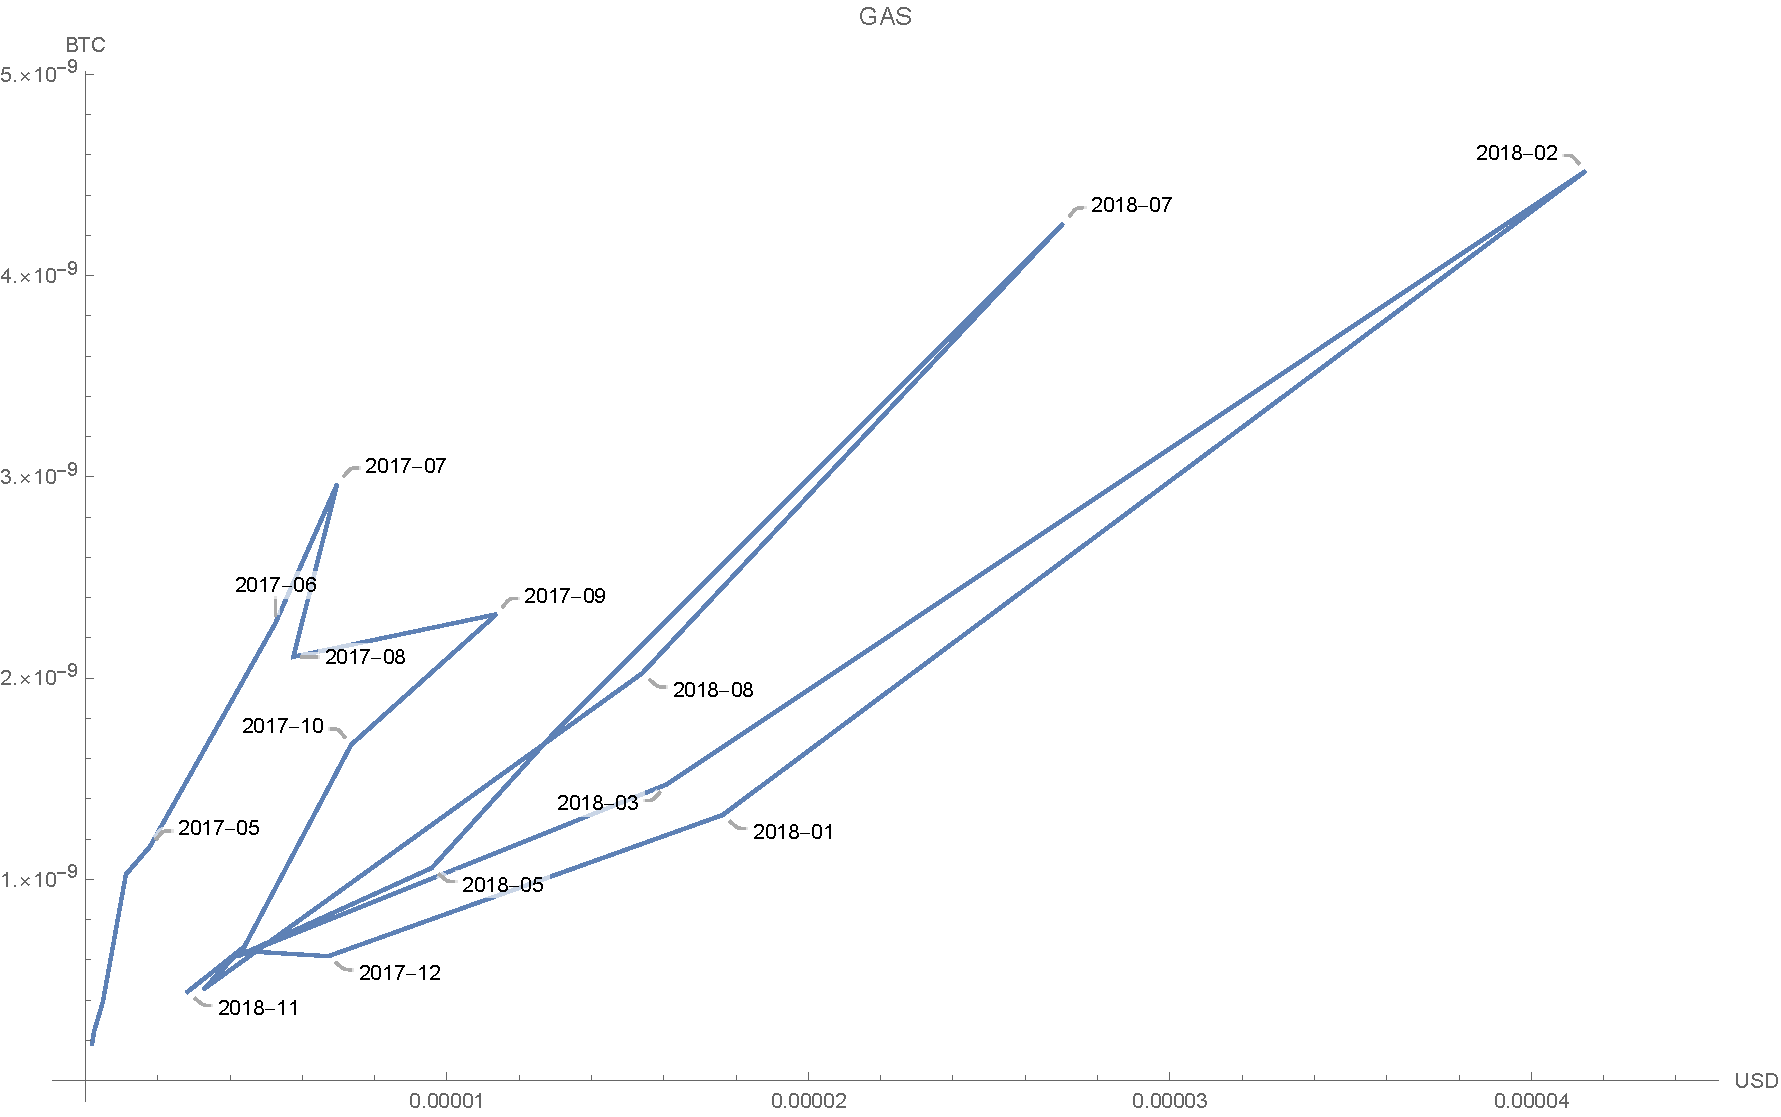
\includegraphics[width=0.45\textwidth]{figures/gas.pdf}\label{fig:gas1}}
	\hfill
	\subfloat[Gas with respect to ETH and Electricity price]{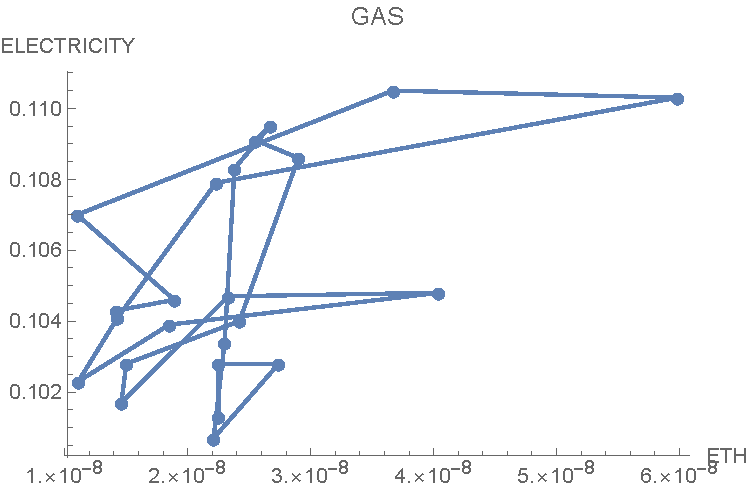
\includegraphics[width=0.45\textwidth]{figures/gasElectricity.pdf}\label{fig:gas2}}
	\caption {Ethereum average GasPrice chart. As mentioned in the Section~\ref{sec:GasInvs}, the two spikes in the chart represent specific events happened in certain dates which have increased the GasPrice.}
	\label{fig:Gas}

\end{figure}

%========================%




\textblue{ Following text should be changed!} \par
Our analysis in Section~\ref{sec:Intro} shows that cryptocurrencies exhibit less stable behavior compared to fiat currencies. Hence, we aim to analyze the price stability of \emph{Gas}. In Ethereum blockchain, every transaction contains a number of operations and there is a precise amount of gas unit associated with each.\footnote{http://ethdocs.org/en/latest/contracts-and-transactions/account-types-gas-and-transactions.html\#what-is-gas} Since Ether is volatile, this concept is introduced to have fixed cost for operations. Thus, even though the price of Ether changes, the amount of Ether corresponding to a unit of gas decreases; so that users pay the same price for the transactions on the Ethereum blockchain. Hence, the notion of gas is yet to be investigated to find out whether it exhibits behavior similar to fiat currencies or cryptocurrencies.

%references to figures wrong now!

Compared to Figure~\ref{fig:eur} and Figure~\ref{fig:eth}, gas plot (Figure~\ref{fig:gas}) has mostly diagonal changes, spread over a smaller range. There are less number of changes compared to ETH. Except from the changes between May 2018-July 2018 and January 2018-March 2018, the gas price changes in a smaller range. Even though there are fluctuations in the gas price, it can be inferred that gas price is less volatile than ETH. Also, it worths mentioning that gas is changing over a small scale in x-axis (USD), when compared to Ether's plot over the same axis in a larger interval.


%==========================================%
\begin{figure}[!htb]
	\centering
	\subfloat[ETH]{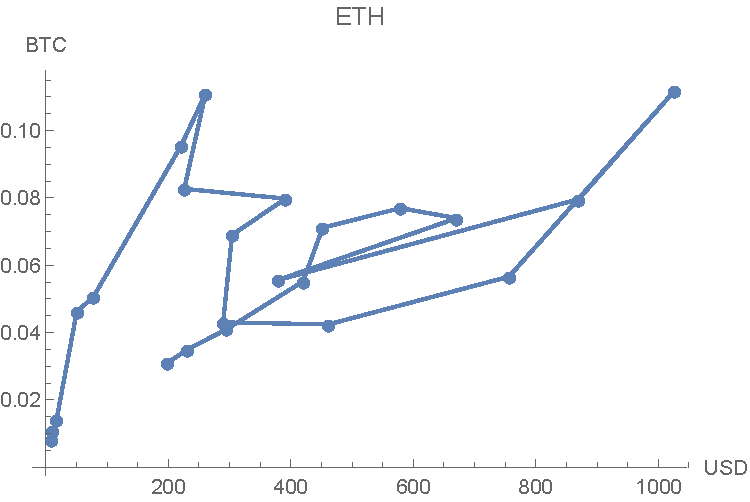
\includegraphics[width=0.45\textwidth]{figures/eth.pdf}\label{fig:cad}}
	\hfill
	\subfloat[XRP]{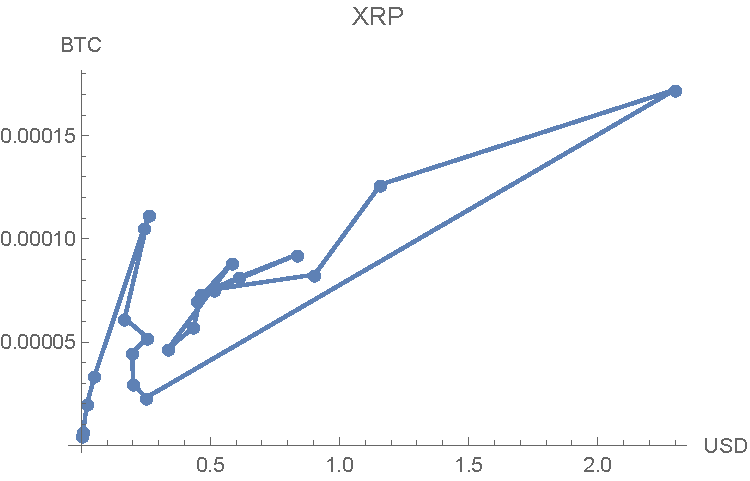
\includegraphics[width=0.45\textwidth]{figures/xrp.pdf}\label{fig:eur}}
	\caption{Volatility in cryptocurrencies}
	\label{fig:fiatandcrypto}
\end{figure}


%========================%

\begin{figure}[!htb]
	\centering
	\subfloat[CAD]{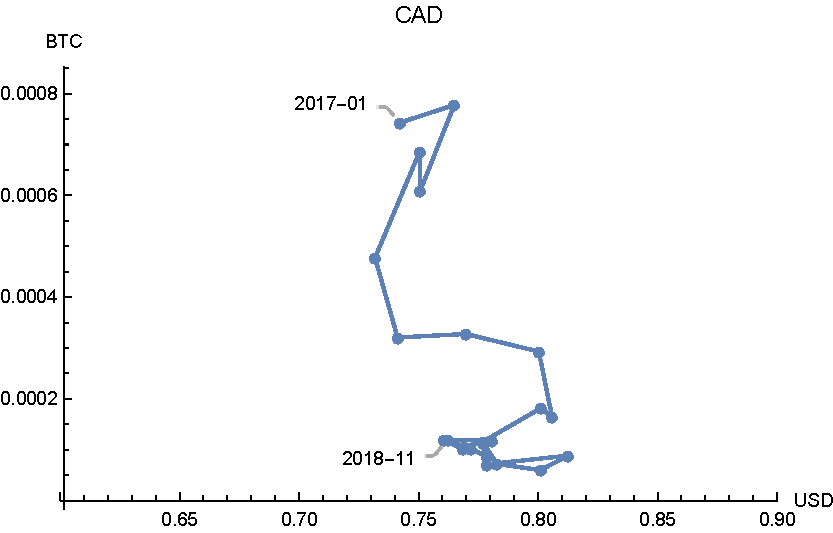
\includegraphics[width=0.45\textwidth]{figures/cad.pdf}\label{fig:cad}}
	\hfill
	\subfloat[EUR]{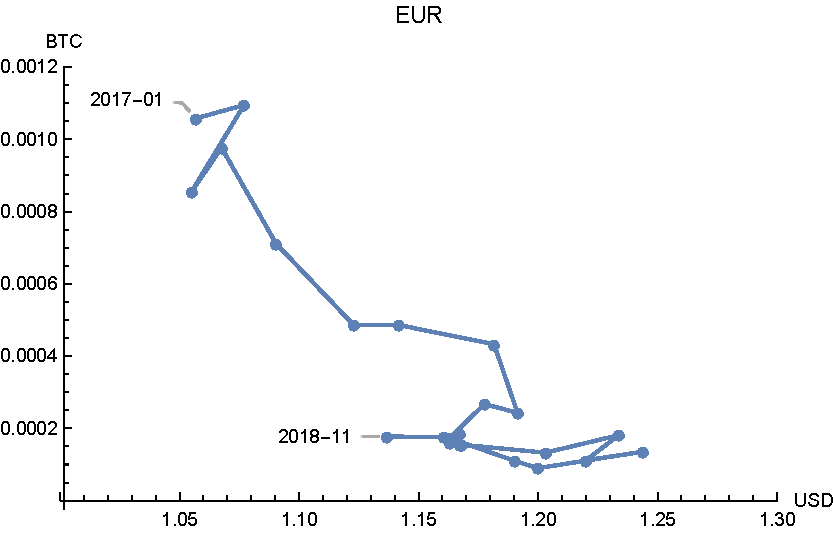
\includegraphics[width=0.45\textwidth]{figures/eur.pdf}\label{fig:eur}}
	\hfill
	\subfloat[Tether]{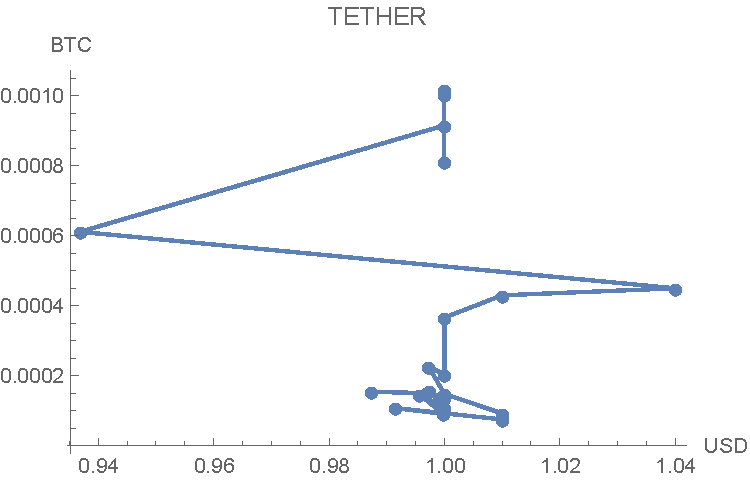
\includegraphics[width=0.45\textwidth]{figures/tether.pdf}\label{fig:tether}}
	\hfill
	\subfloat[BitUSD]{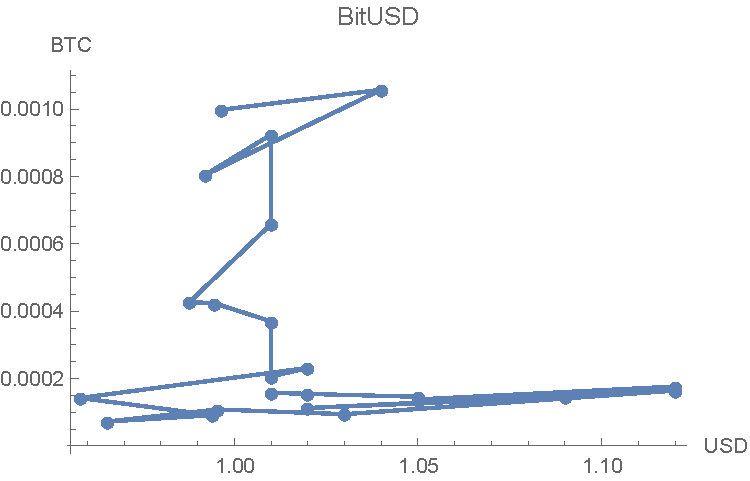
\includegraphics[width=0.45\textwidth]{figures/bitusd.pdf}\label{fig:bitusd}}
	\caption{Stability in two government-issued fiat currencies (CAD and EUR) and two stablecoin projects (Tether and BitUSD). Note that the x-axis is sized consistently across all four plots, with a \$0.30 USD spread. }
	\label{fig:fiatandcrypto}
\end{figure}





%===============

%GRAPHS:
% Figure4: ETH,XRP - (BTC and USD): mostly diagonal movements. Do they move with BTC or not? Shows how cryptocurrencies are volatile. They don't move with BTC
%Figure5: In Figure~\ref{fig:fiatandcrypto}, CAD and EUR are plotted against two reference currencies: BTC on y-axis and USD on x-axis to illustrate what type of movements government issued fiat currencies exhibit. Similarly, two stablecoins, Tether and BitUSD, are also plotted against the same reference currencies.
%CAD, EUR,Tether, BitUsd: We expect stablecoins to be close to a vertical line. CAD and EUR are central bank issued "stablecoins" and compared to Tether and BitUsd (crypto stableoins), we can conclude that they are also fairly stable. (same x-axis range!)The graph seems like Tether's having drastic fluctuations. Note that the price change is around 10 cents. The change is accentuated due to the scale.

%Look at the following paragraph, previous text!
%EUR plot in Figure~\ref{fig:eur} tends to have more movements in the directions 1-5 and 3-7 suggesting that while the value of EUR stays the same according to one axis, it changes according to the other.EUR-USD exchange rate is going under less change, whereas BTC-EUR rate is subject to high volatility.ETH plot in Figure~\ref{fig:eth} illustrates more volatility against BTC and USD, as there are horizontal, vertical and diagonal changes. The fact that the points are spread in a large range of values indicates drastic changes in ETH price with respect to BTC and USD.

% TETHER: Does it artificially inflate BTC price? Do they issue un-backed tokens to reinforce BTC price, then sell BTC to fully back tokens?
%TETHER ATTACK: On October 15, 2018, tether, the market dominating stablecoin with a market cap of $2 billion, was attacked, breaking tether’s peg to USD, dropping its value by 7 percent but simultaneously driving up bitcoin and the whole crypto market by more than 10 percent.
%on October 15, 2018; where the price drastically surged from $6,376 at 12.31 UTC to $7,083 at 14.50 UTC. A downturn in price was seen approximately one hour after that to $6,821, before went stable at around $6,400 — $6,600. It was one of the one of the most unexpected fluctuations after a while. The first ‘stable coin’ tether (USDT) which supposedly pegged 1:1 to the U.S. dollar fell up to 15% at the same time as the price of bitcoin fluctuate wildly. The movement caused a loss of trust among traders, causing them to sell tether and invest in other cryptocurrencies. A massive selloff for tether against bitcoin was seen, resulting in a price rise in bitcoin.
%bitcoin and other crypto assets are perfectly negatively correlated with stablecoins.
%speculative attack

% When tether breaks its peg it moves diagonally, indpendent of bitcoin. When BitUSD breaks, it moves with Bitcoin.

% Talk about Ripple surge in  December 2017 {https://www.forbes.com/sites/jessedamiani/2017/12/22/5-reasons-why-the-ripple-price-is-going-up-so-fast-will-the-xrp-surge-continue/#58337c997cbb}  reasons: altcoins gained importance, Rippe's strategy on partnership and customer acquisition, Ripple's partnersips in Asia, rumors that Coinbase will support xrp, "it's speed (4-second transactions) and low fees also make it appealing to general consumers"

\subsection{Consequences for Central Banking}

\section{Conclusion and Discussion}
In this paper, we analyze the current state of stablecoins with the various options that have been so far proposed to achieve price stability. We also discuss various issues that stablecoins would address. According to the charts represented in the paper, gas is relatively stable in price, while Bitcoin and Ether show volatile behaviour. The reason could be the fact that how users interact with the interface to set the gas price when sending transactions to the Ethereum. By analyzing the properties of gas together with the existing methods to create stablecoin, we can later propose what properties stablecoins should attain.

%==========================================%
